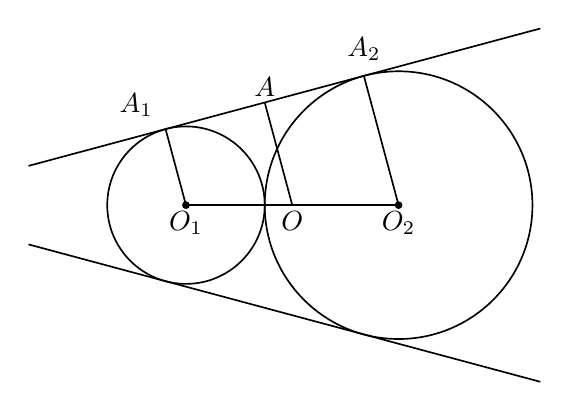
\begin{tikzpicture}[x=1cm,y=1cm,line width=.6pt,font=\normalsize]
\coordinate (O1) at (0,0);
\coordinate (O) at (1.35,0);
\coordinate (O2) at (2.7,0);
\coordinate (A1) at (-0.259259,0.965808);
\coordinate (A) at (1.000000,1.303840);
\coordinate (A2) at (2.259259,1.641873);
\coordinate (T1) at (-2.0,0.498527);
\coordinate (T2) at (4.5,2.243373);
\coordinate (L1) at (-2.0,-0.498527);
\coordinate (L2) at (4.5,-2.243373);
\draw (O1) circle[radius=1.0cm];
\draw (O2) circle[radius=1.7cm];
\draw (T1)--(T2);
\draw (L1)--(L2);
\draw (O1)--(O2);
\draw (O1)--(A1);
\draw (O)--(A);
\draw (O2)--(A2);
\node[below=2pt,inner sep=0pt] at (O1) {$O_{1}$};
\node[below=2pt,inner sep=0pt] at (O) {$O$};
\node[below=2pt,inner sep=0pt] at (O2) {$O_{2}$};
\node[above left=1pt] at (A1) {$A_{1}$};
\node[above=2pt,inner sep=0pt] at (A) {$A$};
\node[above=2pt] at (A2) {$A_{2}$};

% Explicit named circle-center points, painted after all region fills.
\fill (O1) circle[radius=1.4pt];
\fill (O2) circle[radius=1.4pt];
\end{tikzpicture}
